\chapter{Tileset}\label{tileset}
	\section{Introduction}
		The tileset is a set of \emph{Tiles}. Each Tileset is built using an image. This image is divided into a set of subimages, each of this subimage is a \emph{Tile}. All Tiles in a tileset are square and have the same size (pixels).
	
	
	\section{Tile}
		Each tile of a Tileset as attributes one image (java.awt.Image) and informations about wich directions the player and enemies can pass in this tile, as shows Figure \ref{fig:tile}.
		
	\begin{figure}[h]
		\centering
		
\includegraphics[]{img/tile.png}
		\caption{Tile: a tile have information about wich directions the player can pass. In this example the player can't pass from up to down.}
		\label{fig:tile}
	\end{figure}

	\section{Tileset}
		A tileset is a set of tiles. An image is loaded and a tile size is set. The image of Tileset is cut into as many as possible Tiles. This set of tiles are used to create an Scenary. Figure \ref{fig:tileset} shows an tileset example.
		\begin{figure}[h]
			\centering
			\subfigure[][]{
\includegraphics[width=5cm]{img/tile_input.png}}
			\qquad
			\subfigure[][]{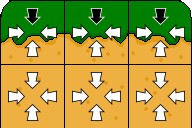
\includegraphics[width=5cm]{img/tile_processed.png}}
			
			\caption{Tileset: the image (a) is cut into various subimages. Each subimage is a \emph{Tile} and have its own attributes.}
		\label{fig:tileset}
	\end{figure}
		
	\section{File Format}
		The tileset can be saved to a file. It is written in binary format, and the format is shown in Listing \ref{listing-tilesetFormat}.
		
		\begin{algorithm}[H]
			\caption{Tileset File Format.}
	      \label{listing-tilesetFormat}
	      \begin{algorithmic}
			\STATE $[int]Number\_tiles\_Y$
			\STATE $[int]Number\_tiles\_X$
			\STATE $[int]Tile\_size$
			
			\FOR{$i=0 \dots Number\_tiles\_Y$}
				\FOR{$j=0 \dots Number\_tiles\_X$}
					\STATE $[int]tile[i][j].terrain\_type$
					\STATE $[bool]tile[i][j].pass\_from\_up$
					\STATE $[bool]tile[i][j].pass\_from\_down$
					\STATE $[bool]tile[i][j].pass\_from\_left$
					\STATE $[bool]tile[i][j].pass\_from\_right$
					\STATE $[int]tile[i][j].image\_height$
					\STATE $[int]tile[i][j].image\_width$
					\FOR{$x=0 \dots tile[i][j].image\_width$}
						\FOR{$y=0 \dots tile[i][j].image\_height$}
							\STATE $[int]tile[i][j].image[x][y]$
						\ENDFOR
					\ENDFOR
				\ENDFOR
			\ENDFOR
		  \end{algorithmic}
		 \end{algorithm}